\documentclass{article}

% Language setting
% Replace `english' with e.g. `spanish' to change the document language
\usepackage[english]{babel}
\usepackage{graphicx}
\graphicspath{ {./Images/} }
\usepackage{caption}
\captionsetup[figure]{font=small}

% Set page size and margins
% Replace `letterpaper' with `a4paper' for UK/EU standard size
\usepackage[letterpaper,top=2cm,bottom=2cm,left=3cm,right=3cm,marginparwidth=1.75cm]{geometry}

% Useful packages
\usepackage{amsmath}
\usepackage{graphicx}
\usepackage[colorlinks=true, allcolors=blue]{hyperref}

\title{Research Proposal: Using Machine Learning to optimize the calibration of Discrete Particle Model}
\author{Q.H. Nguyen\\[1ex] \small Head Supervisor: Thomas Weinhart, Daily Supervisor: Anthony Thornton, Additional member: Chen Kuan.} 
\date{}

\begin{document}
\maketitle

\section{Introduction}


\subsection{Granular Material}

 Granular material is a family of material characterized by its large bulk of densely packed particles, ranging from nanometers to centimeters \cite{introGranular2}, and is able to resist deformation and form heaps \cite{introGranular3}, i.e., behave like a solid and withstand strong shear force. Simple examples of granular materials include sand, gravel, clays, seeds, nuts, and all ranges of powders such as coffee powder, cement powder. Furthermore, many processes and equipments in chemical plants use granular materials, such as catalysis, adsorption, and heat exchangers. Granular materials are projected to make about half of the products and three-quarters of the raw materials used in the chemical industry \cite{introGranular}. Thus, understanding how granular materials behave is of great significance.




\subsection{Discrete Particle Model and calibration}

Granular material's bulk behavior is simulated using a Discrete Particle Model (DPM, or Discrete Element Method - DEM), which generates the movement of individual particles to capture the macro-scale behavior. The DPM is a family of numerical methods for computing the motion of a large number of particles \cite{Weng:2015}. Since the properties of granular materials differ wildly, these simulations require an extensive calibration process designed individually for each type of granular material. Some parameters of the granular material model can be measured directly, such as size distribution or density. However, other parameters are effective parameters (i.e., they result from a simplified particle model) and thus cannot be directly measured. These parameters are then calibrated by choosing a few standard calibration setups (rotating drum, heap test, ring shear cell) and simulating these setups in a DPM simulation, and the missing parameters are determined such that the response of the experimental and simulation setups match. This has been done using a Convolutional Neural Network \cite{nn-calibration} and Genetic Algorithm \cite{ga-calibration}. However, these methods are very costly in terms of  time and resources, since it requires a large number of DEM simulations. In this research assignment, another algorithm will be studied: GrainLearning - a Python-based Bayesian calibration tool developed by H.Cheng et al. \cite{grainLearning}. GrainLearning utilizes the recursive Bayesian algorithm to estimate the uncertainty parameters in DPM. As mentioned above, each model requires extensive calibration, and using GrainLearning can make the calibration process more effective by iteratively searching for the optimized parameters, effectively reduce the number of DEM simulation required.

\subsection{Goals of the Assignment}

GrainLearning has been implemented in MercuryDPM and produces satisfactory results in many cases. However, it is far from clear whether the chosen optimization algorithm is optimal, i.e., whether the calibration results in an optimal parameter set and whether the optimum could be reached faster, since currently, a calibration process could run for hours. Therefore, the main goal of the research is to study, analyse, and improve the calibration process of the GrainLearning algorithm, and further experimental procedure to archieve this goal will be described in the experimental section below. 

\begin{figure}
    \centering
    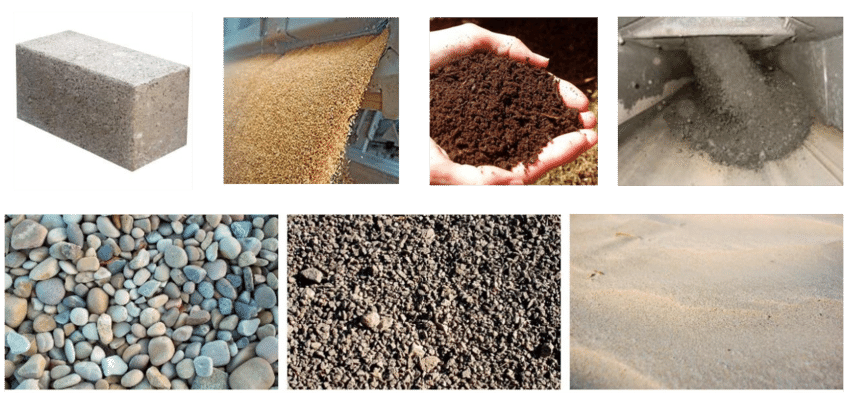
\includegraphics[scale=0.5]{granularExample.png}
    \caption{Examples of Granular Materials.\cite{granularExample}}
    \label{fig:granularExample}
\end{figure}

\section{Timeline and procedure}
\begin{figure}
    \centering
    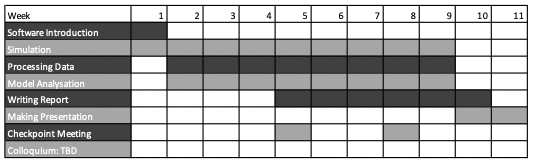
\includegraphics[scale=0.8]{timeline.png}
    \caption{Timeline of the Assignment}
    \label{fig:timeline}
\end{figure}

The timeline of the assignment is described in figure \ref{fig:timeline}. In the first week, I will spend time working on different tutorials of MercuryDPM, to get myself familiar with the software. I will also look into the source code of GrainLearning, study the structure and the mathematics of the algorithm. In the coming weeks (up to and including week 9), different simulations will be carried out as part of the experiment on MercuryDPM, initially using a synthesized data with simplified number of parameters (start with 2: sliding friction and restitution). To collect the bulk parameters, two type of experiments will be performed: Rotating drum and heap test. The corresponding data will then be passed through to assess the ability of GrainLearning in calibrating the sliding friction and restitution. The report will be start as soon as I obtained positive experimental results, which is projected to be after week 4. However, during the assignment, I will be keeping a journal and agendas of all meeting to document the process.  

\pagebreak
\bibliographystyle{elsarticle-num}
\bibliography{citation}

\end{document}